%%%%%%%%%%%%%%%%%%%%%%%%%%%%%%%%%%%%%%%%%%%%%%%%%%%%%%%%%%%%%
%% Begin exercise %%
%%%%%%%%%%%%%%%%%%%%%%%%%%%%%%%%%%%%%%%%%%%%%%%%%%%%%%%%%%%%%
\ex{Rectifiers}

%%%%%%%%%%%%%%%%%%%%%%%%%%%%%%%%%%%%%%%%%%%%%%%%%%%%%%%%%%%%%
%% Task 1: B2U topology with capacitive filtering %%
%%%%%%%%%%%%%%%%%%%%%%%%%%%%%%%%%%%%%%%%%%%%%%%%%%%%%%%%%%%%%
\task{B2U topology with capactive filtering}
An uncontrolled single-phase, two-pulse rectifier circuit with capacitive filtering 
is shown in \autoref{fig:B2U_Topology_Cap_Filtering}.
All components, including the diodes, are assumed to be ideal. On the input side, 
the single-phase AC supply with voltage $u_\mathrm{1}(t)$ is connected, while on the output side, 
a smoothing capacitor $C$ and a constant current load $I_\mathrm{0}$ are present.

%%%%%%%%%%%%%%%%%%%%%%%%%%%%%%%%%%%%%%%%%%%%%%%%%%%%%%%%%%%%%%%%%%%%%%%
 % B2U rectifier with capacitive output filtering
%%%%%%%%%%%%%%%%%%%%%%%%%%%%%%%%%%%%%%%%%%%%%%%%%%%%%%%%%%%%%%%%%%%%%%%
    \begin{figure}[htb]
        \begin{center}
            \begin{circuitikz}[european currents,european resistors,american inductors]
                \draw
                % Base point for voltage supply
                (0,0) coordinate (jU1v)
                % Add supply U1 [open, o-o, v = $u_1(t)\hspace{0.5cm}$, voltage = straight]
                (jU1v) to [open, o-o, v = $u_1(t)\hspace{0.5cm}$, voltage = straight] ++(0,-2) coordinate (jU1g)
                % Add arrow and Text
                (jU1v) ++(0.5,0) node[currarrow](I1){}  
                (I1)  node[anchor=south,color=black]{$i_\mathrm{1}(t)$}  
                % Add connection to diode D1/D4
                (jU1v) to [short, -*] ++(2,0) coordinate (jaD1)
                % Add D1 
                (jaD1) to [diode, l=$D_1$]  ++(0,1.5)  coordinate (jkD1)
                % Add D4 connection S
                (jaD1)  ++(0,-3.5)  coordinate (jaD4)
                % Add D4 
                (jaD4) to [diode, l=$D_4$] ++(0,1.5)  coordinate (jkD4)
                % Add connection D4 to D1
                (jkD4) to [short, -]  (jaD1)
                % Add connection to diode D3/D2
                (jU1g) to [crossing, -*, mirror] ++(4,0)  coordinate (jkD2)
                % Add connection D2 to D3
                (jkD2) to [short, -] ++(0,2) coordinate (jaD3)
                % Add D3 
                (jaD3) to [diode, l=$D_3$]  ++(0,1.5)  coordinate (jkD3)
                % Add D2 connection 
                (jkD2)  ++(0,-1.5)  coordinate (jaD2)
                % Add D2 
                (jaD2) to [diode, l=$D_2$] (jkD2)
                % Add connection D1 to D3
                (jkD1) to [short, -*] (jkD3)                
                % Add connection to capacitor plus
                (jkD3) to [short, -*, i=$i_2(t)$] ++(2,0) coordinate (jvCp)
                % Add connection to current source vI0
                (jvCp) to [short, -] ++(1.5,0) coordinate (jvI0)
                % Add coordinate of current source gI0
                (jvI0) ++(0,-5) coordinate (jgI0)
                % Add current source I0
                (jvI0) to [isource, l=$I_0$] (jgI0)
                % Add connection to capacitor minus
                (jgI0) to [short, -*] ++(-1.5,0) coordinate (jgCm)
                % Add capacitor
                (jvCp) to [C, v= $u_\mathrm{2}(t)$, voltage = straight, l=$C$, i=${i_\mathrm{C}(t)}$] (jgCm)
                % Add connection to D2
                (jgCm) to [short, -*] (jaD2)
                % Add connection D2 to D4
                (jaD2) to [short, -] (jaD4);
            \end{circuitikz}
    \end{center}
        \caption{B2U rectifier with capacitive output filtering.}
        \label{fig:B2U_Topology_Cap_Filtering}
    \end{figure}




\begin{table}[ht]
    \centering  % Zentriert die Tabelle
    \begin{tabular}{llll}
        \toprule
        
        Input voltage: &  $u_\mathrm{1}(t) = \SI{156}{\volt}\cdot \sin(\omega t)$ & Load current: & $I_{\mathrm{0}} = \SI{7.5}{\ampere}$ \\ 
        Filter capacitance: & $C = \SI{330}{\micro\farad}$  & Frequency: & $f= \SI{60}{\hertz}$ \\ 
        \bottomrule
    \end{tabular}
    \caption{Parameters of the B2U rectifier.}  
    \label{table:ex05_Parameters of the circuit}
\end{table}

The angle $\alpha$ represents the phase angle range between zero crossing of the supply voltage and the phase angle
at which all four diodes are blocked, meaning the capacitor discharges through the load. The angle $\beta$ 
represents the phase angle range between $\alpha$ and the phase angle at which two of the four diodes begin to 
conduct, i.e., when the capacitor is recharged from the mains supply.
A steady-state operation is assumed for this task.

\subtask{Calculate the two angles $\alpha$ and $\beta$.
Note: For the calculation of $\beta$ you can use the following simple approximation: $\sin(x) \approx x$.
(This approximation is sufficiently accurate within a range of approximately $x=\pm \SI{25}{\degree}$.)}
\begin{solutionblock}
    As long as the voltage $\left| u_\mathrm{1}(t) \right|$ increase the voltage $u_\mathrm{2}(t)$ of the capacitor follows:
    \begin{equation} 
        u_\mathrm{2}(t) = \left| \hat{u}_\mathrm{1}\sin(\omega t)\right|.
    \end{equation}
    If the capacitor supplies the load current $I_\mathrm{0}$ the voltage $u_\mathrm{2}(t)$ at the capacitor 
    decreases linear with:
    \begin{equation} 
        dU_\mathrm{C}(t)=\frac{d(u_\mathrm{2}(t))}{dt} = -\frac{I_\mathrm{0}}{C}=-\frac{\SI{7.5}{\ampere}}{\SI{330}{\micro\farad}}
        =-\SI{22.7}{\kilo\volt/\second}.
        \label{eq:deltaVoltageAtCapacitorA_ex05}
    \end{equation} 
    If the voltage $u_\mathrm{2}(t)$ decreases faster than $d(u_\mathrm{2}(t))/dt$
    then all diodes blocks and the capacitor supplies the current load $I_\mathrm{0}$. This leads to:
    \begin{equation} 
        \frac{d(u_\mathrm{2}(t))}{dt} = \frac{d(\left| \hat{u}_\mathrm{1}\sin(\omega t)\right|)}{dt} 
        = \omega\left| \hat{u}_\mathrm{1}\cos(\omega t)\right| = -\frac{I_\mathrm{0}}{C}.
        \label{eq:deltaVoltageAtCapacitorB_ex05}
    \end{equation} 
    Solving \eqref{eq:deltaVoltageAtCapacitorB_ex05} with respect to $\omega \cdot t = \alpha$ yields
    \begin{equation}
        \alpha = \arccos(-\frac{I_\mathrm{0}}{\omega C \cdot \hat{u}_\mathrm{1}})
        = \arccos(-\frac{\SI{7.5}{\ampere}}{2 \pi \cdot \SI{60}{\hertz} \cdot \SI{330}{\micro\farad} \cdot \SI{156}{\volt}}) = \SI{112.8}{\degree}.
    \end{equation}
    The capacitor is discharging by the load  $I_\mathrm{0}$ at $\alpha$, which corresponds to a 
    voltage of: 
    \begin{equation}
        \hat{u}_\mathrm{1}\sin(\omega t) = \hat{u}_\mathrm{1}\sin(\alpha) 
        = \SI{156}{\volt} \cdot \sin(\SI{112.8}{\degree})=\SI{143.4}{\volt}.
    \end{equation}    
    In that moment when the voltage $\left| u_\mathrm{1}(t) \right|$ becomes equal to $u_\mathrm{2}(t)$ 
    the discharge of the capacitor stops and $u_\mathrm{2}(t)$ follows again $\left| u_\mathrm{1}(t) \right|$.
    The voltage $\left| \hat{u}_\mathrm{1}(t) \right|$ increases again at $\pi$ with:
    \begin{equation}
        \left| \hat{u}_\mathrm{1}\sin(\omega t + \pi ) \right| = \hat{u}_\mathrm{1}\sin(\omega t) \quad \text{for} \quad t \leq \pi.
    \end{equation}
    If we consider $t=0$ as the point in time at which the voltage $u_\mathrm{2}(t)$ begins to rise, the following 
    results compared to the previous point in time at which the capacitor begins to discharge:      
    \begin{equation}
        t_\mathrm{\alpha}=\frac{\pi - \alpha_\mathrm{rad}}{\omega} = 
        \frac{\pi - \SI{1.969}{\radian}}{\SI{377}{\hertz}} = \SI{-3.111}{\milli\second}
    \end{equation}   
    With the approximation $\sin(x) = x$ we get
    \begin{equation}
        \hat{u}_\mathrm{1}\sin(\alpha) + dU_\mathrm{C}(t) \cdot (t-t_\mathrm{\alpha}) = \hat{u}_\mathrm{1}\cdot \omega t.
        \label{eq:stopCapacitordischarge_ex05}
    \end{equation}   
    Solving \eqref{eq:stopCapacitordischarge_ex05} with respect to $\omega t$ leads to
    \begin{equation}
        \omega t = \frac{\hat{u}_\mathrm{1}\sin(\alpha) - dU_\mathrm{C}(t) \cdot t_\mathrm{\alpha}}
                   {\hat{u}_\mathrm{1}-\frac{dU_\mathrm{C}(t)}{\omega}}=
                   \frac{\SI{143.4}{\volt} - \SI{22.7}{\kilo\volt/\second} \cdot \SI{3.111}{\milli\second}}
                   {\SI{156}{\volt}-\frac{\SI{22.7}{\kilo\volt/\second}}{\SI{377}{\hertz}}}=\SI{0.337}{\radian}.
    \end{equation}
    $\beta$ is to calculate by distance between $\alpha$ and the calculated $\omega t$:
    \begin{equation}
        \beta=\omega t + \pi - \alpha = \SI{0.337}{\radian} + \pi - \SI{1.969}{\radian}
        = \SI{1.51}{\radian} = \SI{86.5}{\degree}.
    \end{equation}
\end{solutionblock}

\vspace{2em}\par
If you were unable to solve task (a), please use $\alpha=\SI{112.8}{\degree}$ and $\beta=\SI{86.5}{\degree}$.

\subtask{Sketch the capacitor voltage $u_\mathrm{2}(\omega t)$ considering $\omega t \in [0,...,2\pi]$ taking 
into account the previously calculated angles $\alpha$ and $\beta$.}
\begin{solutionblock}
    \autoref{sfig:ex05_Voltage_u2_andCurrent_i1_ic} displays the voltage at the capacitor.
    %%%%%%%%%%%%%%%%%%%%%%%%%%%%%%%%%%%%%%%%%%%%%%%%%%%%%%%%%%%%%%%%%%%%%%%%%%
% Signals of U2 and i1 and i2
%%%%%%%%%%%%%%%%%%%%%%%%%%%%%%%%%%%%%%%%%%%%%%%%%%%%%%%%%%%%%%%%%%%%%%%%%%
\begin{solutionfigure}[htb]

 %   \documentclass{standalone}
 %   \usepackage{pgfplots}
 %   \pgfplotsset{compat=1.18} % Kompatibilität für neuere Versionen
        \centering
        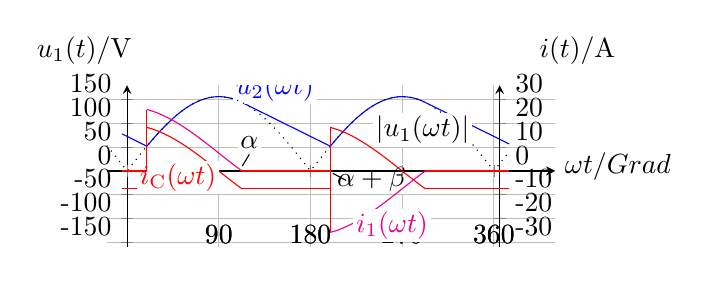
\begin{tikzpicture}
            \begin{axis}[
                    % x/y range adjustment
                    xmin=-20, xmax=420,
                    ymin=-160, ymax=180,
                    samples=500,
                    axis y line=center,
                    axis x line=middle,
                    extra y ticks=0,
                    % Label text
                    xlabel={$\omega t / \text{Grad}$},,
                    ylabel={$u_\mathrm{1}(t)/\mathrm{V}$},
                    % Label adjustment
                    x label style={at={(axis description cs:1,0.5)},anchor=west},
                    y label style={at={(axis description cs:-.05,.97)},anchor=south,yshift=0.2cm},
                    width=0.6\textwidth,
                    height=0.3\textwidth,
                    % x-Ticks
                    xtick={0,90,180,270,360},
                    xticklabels={,90,180,270,360},
                    xticklabel style = {anchor=north,yshift=-0.5cm},
                    % y-Ticks
                    ytick={150,100,50,-50,-100,-150},
                    yticklabels={150,100,50,-50,-100,-150},
                    yticklabel style = {yshift=0.2cm,anchor=east},
                    % Grid layout
                    grid,
                    %grid style={line width=.1pt, draw=gray!10},
                    %major grid style={line width=.2pt,draw=gray!90},
                ]
                % Voltage u2(wt) if supplied by u1(wt)
                \addplot[blue, domain= 19.3:112.8] {abs(156*sin(x))};                
                \addplot[blue, domain= 199.3:292.8] {abs(156*sin(x))};                
                % Voltage u2(wt) if supplied by uc(wt)
                \addplot[blue, domain=-5:19.3] {143.8-(x+67.2)*1.06};                
                \addplot[blue, domain=112.8:199.3] {143.8-(x-112.8)*1.06};                
                \addplot[blue, domain=292.8:375] {143.8-(x-292.8)*1.06};
                % Label of u2
                \node[blue, fill=white, inner sep = 1pt, anchor = south] at (axis cs:145,140) {$u_{\mathrm{2}}(\omega t)$};
                % Voltage u1(wt)
                \addplot[black, domain= -20:375,dotted] {abs(156*sin(x))};                
                % Label of u2
                \node[black, fill=white, inner sep = 1pt, anchor = south] at (axis cs:290,50) {$\left|u_{\mathrm{1}}(\omega t)\right|$};
                % Label of alpha
                \node[black, fill=white, inner sep = 1pt, anchor = south] at (axis cs:120,40) {$\alpha$};
                % Line to axes for alpha
                \draw[thin, black] (120,35) -- (113,10);
                % Label of alpha + beta
                \node[black, fill=white, inner sep = 1pt, anchor = south] at (axis cs:240,-50) {$\alpha+\beta$};
                % Line to axes for beta
                \draw[thin, black] (215,-20) -- (202,-5);

            \end{axis}     
            \begin{axis}[
                % x/y range adjustment
                xmin=-20, xmax=420,
                ymin=-32, ymax=36,
                samples=500,
                axis y line=right,
                axis y line shift=-20pt,
                axis x line=middle,
                extra y ticks=0,
                % Label text
                ylabel={$i(t)/\mathrm{A}$},
                % Label adjustment
                y label style={at={(axis description cs:1.05,.97)},anchor=south, rotate=270,yshift=0.2cm},
                width=0.6\textwidth,
                height=0.3\textwidth,
                % x-Ticks
                xtick={0,90,180,270,360},
                xticklabels={,90,180,270,360},
                xticklabel style = {anchor=north,yshift=-0.5cm},
            % y-Ticks
                ytick={30,20,10,-10,-20,-30},
                yticklabels={30,20,10,-10,-20,-30},
                yticklabel style = {yshift=0.2cm,anchor=west},
                % Grid layout
                % grid=both,
                % grid style={line width=.1pt, draw=gray!10},
                % major grid style={line width=.2pt,draw=gray!90},
            ]
                % Current ic(t)
                \addplot[red, domain= 19.3:112.8] {19.4*cos(x)};                
                \addplot[red, domain= 199.3:292.8] {-19.4*cos(x)};                
                % Current ic(t) if supplied by uc(t)
                \addplot[color=red,mark=none,solid] coordinates{
                    (-5, -7.5)
                    (19.3, -7.5)
                    (19.3,18.3)
                    }; 
                \addplot[color=red,mark=none,solid] coordinates{
                    (112.8, -7.5)
                    (199.3, -7.5)
                    (199.3,18.3)
                    }; 
                \addplot[color=red,mark=none,solid] coordinates{
                    (292.8, -7.5)
                    (375, -7.5)
                     }; 
                % Label of ic
                \node[red, fill=white, inner sep = 1pt, anchor = south] at (axis cs:50,-10) {$i_{\mathrm{C}}(\omega t)$};

                % Current i1(wt)
                \addplot[magenta, domain= 19.3:112.8] {19.4*cos(x)+7.5};                
                \addplot[magenta, domain= 199.3:292.8] {19.4*cos(x)-7.5};                
                % Current i1(wt) if supplied by uc(t)
                \addplot[color=red,mark=none,solid] coordinates{
                    (-5,0)
                    (19.3,0)
                    (19.3,25.8)
                    }; 
                \addplot[color=red,mark=none,solid] coordinates{
                    (112.8,0)                    
                    (112.8,0)
                    (199.3,0)
                    (199.3,-25.8)
                    }; 
                \addplot[color=red,mark=none,solid] coordinates{
                    (292.8,0)                    
                    (292.8,0)
                    (375,0)
                    }; 
                % Label of i1
                \node[magenta, fill=white, inner sep = 1pt, anchor = south] at (axis cs:260,-30) {$i_{\mathrm{1}}(\omega t)$};
            \end{axis}
        \end{tikzpicture}
        \caption{Voltage at primary side.}
        \label{sfig:ex05_Voltage_u2_andCurrent_i1_ic}
\end{solutionfigure}  
\end{solutionblock}

\subtask{Calculate the currents $i_\mathrm{1}(\omega t)$  and $i_\mathrm{C}(\omega t)$ and and add them to the previous plot.}
\begin{solutionblock}
    For current of $i_\mathrm{1}(\omega t)$ and  $i_\mathrm{C}(\omega t)$ two cases are to consider. If $\alpha<\omega t<\alpha+\beta$
    and $\pi+\alpha<\omega t<\pi+\alpha+\beta$,the capacitor supplies the load current $I_{\mathrm{0}}$.
    The remaining phase angle range the input voltage supplies the current load $I_{\mathrm{0}}$ and charge the capacitor.
    For $\alpha<\omega t<(\alpha+\beta)$ and $(\pi+\alpha)<\omega t<(\pi+\alpha+\beta)$ the current $i_\mathrm{C}(\omega t)$ 
    corresponds to the current $-I_{\mathrm{0}}$ while all diodes are inactive.
    \begin{equation} 
        i_\mathrm{C}(\omega t)=-I_{\mathrm{0}} \quad \text{and} \quad i_\mathrm{1}(\omega t)= i_\mathrm{2}(\omega t)= \SI{0}{\ampere}
    \end{equation}
    For $(\alpha+\beta-\pi)\leq\omega t\leq\alpha$ and $(\alpha+\beta)\leq\omega t\leq(\pi+\alpha)$ the current $i_\mathrm{C}(\omega t)$ results in:
    \begin{equation} 
        i_\mathrm{C}(\omega t)=C\frac{d(u_\mathrm{2}(t))}{dt}=C\frac{d(\left| \hat{u}_\mathrm{1}\sin(\omega t)\right|)}{dt}
        = \omega C \left|\hat{u}_\mathrm{1}\cos(\omega t)\right| 
    \end{equation}
    Entering numbers leads to
    \begin{equation} 
        i_\mathrm{C}(\omega t)= \SI{377}{\hertz} \cdot \SI{330}{\micro\farad} \cdot  \left|\SI{156}{\volt}\cos(\omega t)\right|
        =\SI{19.4}{\ampere}\left| \cdot \cos(\omega t)\right| 
    \end{equation}
    The current $i_\mathrm{2}(\omega t)$ is the sum of $I_{\mathrm{0}}$ and $i_\mathrm{C}(\omega t)$.
    \begin{equation} 
        i_\mathrm{2}(\omega t)=i_\mathrm{C}(\omega t) + I_{\mathrm{0}}=\SI{19.4}{\ampere}\left|\cos(\omega t)\right| + \SI{7.5}{\ampere}
    \end{equation}
    The current $i_\mathrm{1}(\omega t)$ depends on the diodes, which are active.
    \begin{align}
        \begin{split}
            i_\mathrm{1}(\omega t)=i_\mathrm{2}(\omega t) \quad \text{for} \quad (\alpha+\beta-\pi)\leq\omega t\leq\alpha \\
            i_\mathrm{1}(\omega t)=-i_\mathrm{2}(\omega t) \quad \text{for} \quad (\alpha+\beta)\leq\omega t\leq\pi+\alpha
        \end{split}
    \end{align}

    The currents $i_\mathrm{C}(\omega t)$ and $i_\mathrm{1}(\omega t)$ are entered in \autoref{sfig:ex05_Voltage_u2_andCurrent_i1_ic}.

\end{solutionblock}

\subtask{Assume the smoothing capacitor is very large, i.e., $C\rightarrow \infty$. What is the average active power $P_\mathrm{0}$ 
absorbed by the current source? What will $P_\mathrm{0}$ be if $C=\SI{330}{\micro\farad}$?}
\begin{solutionblock}
    Considering \eqref{eq:deltaVoltageAtCapacitorA_ex05} a very large capacitor leads to a very low voltage decrease. It means for
    a capacitor with $C\rightarrow \infty$ the voltage decrease is zero and $u_\mathrm{2}(\omega t)=\hat{u}_\mathrm{1}$. 
    In this case the power, which the current load absorbed results in
    \begin{equation} 
        P_\mathrm{0}=\hat{u}_\mathrm{1} \cdot I_{\mathrm{0}}=\SI{156}{\volt}\cdot\SI{7.5}{\ampere}=\SI{1167}{\watt}.
    \end{equation}
    For the capacitor with \SI{330}{\micro\farad} again the two phase angle ranges are to consider. For the phase angle range
    $(\alpha+\beta-\pi)\leq\omega t\leq\alpha$. To simplify the calculation, the minimal phase angle is expressed as:
    \begin{equation} 
        \beta'=\alpha+\beta-\pi=\SI{1.969}{\radian}+\SI{1.51}{\radian}-\pi
        =\SI{0.337}{\radian} = \SI{19.3}{\degree}.
    \end{equation}
    Using $\beta'$ the absorbed average power of the current load is calculated by:
    \begin{equation} 
        P_\mathrm{0,1}=\frac{\hat{u}_\mathrm{1} \cdot I_{\mathrm{0}} \cdot \omega}{\alpha-\beta} \int_{\beta'}^{\alpha} \sin(\omega t) dt
    \end{equation}
    This leads to
    \begin{equation} 
        P_\mathrm{0,1}=\frac{\hat{u}_\mathrm{1} \cdot I_{\mathrm{0}}}{\alpha-\beta} \left( \cos(\beta') - \cos(\alpha) \right)
    \end{equation}
    Entering numbers leads to
    \begin{equation} 
        P_\mathrm{0,1}=\frac{\SI{156}{\volt} \cdot \SI{7.5}{\ampere}}{\SI{1.969}{\radian}-\SI{0.337}{\radian}}
         \left( \cos(\SI{0.337}{\radian}) - \cos(\SI{1.969}{\radian}) \right)=\SI{952}{\watt}.
    \end{equation}
    For the phase angle range $\alpha<\omega t<(\alpha+\beta)$ the absorbed average power of the current load is calculated by:
    \begin{equation} 
        P_\mathrm{0,2}=\hat{u}_\mathrm{1} \cdot I_{\mathrm{0}} \frac{\sin(\alpha) + \sin(\beta')}{2}=
        \SI{156}{\volt} \cdot \SI{7.5}{\ampere} \cdot \frac{\sin(\SI{112.8}{\degree}) + \sin(\SI{19.3}{\degree})}{2}=
        \SI{733}{\watt}
    \end{equation}
    The total absorbed average power of the current load results from the weighted sum of $P_\mathrm{0,1}$ and $P_\mathrm{0,2}$:
    \begin{equation} 
        P_\mathrm{0}=\frac{(\SI{180}{\degree}-\beta) \cdot P_\mathrm{0,1}+ \beta \cdot P_\mathrm{0,2}}{\SI{180}{\degree}}
        =\frac{(\SI{180}{\degree}-\SI{86.5}{\degree}) \cdot \SI{952}{\watt}+\SI{86.5}{\degree} \cdot \SI{733}{\watt}}{\SI{180}{\degree}}=\SI{847}{\watt}
    \end{equation}
    
\end{solutionblock}

\subtask{What is the minimum blocking voltage ratings of the diodes to ensure that the rectifiers is not damaged?}
\begin{solutionblock}
    The voltage supply causes a voltage  potential shift of $u_\mathrm{1}(t)$ at it's two connection points. 
    The maximal potential difference occurs at $\hat{u}_\mathrm{1,pm}=\pm \SI{156}{\volt}$.
    The sum of the voltage drop across $D_\mathrm{1}$ and $D_\mathrm{4}$ at the first branch and $D_\mathrm{3}$ and $D_\mathrm{2}$
    at the second branch corresponds to $u_\mathrm{2}(t)$ with a maximal value of $\hat{u}_\mathrm{2}=\SI{156}{\volt}$. 
    This leads to a maximal blocking voltage for $D_\mathrm{3}$ and $D_\mathrm{4}$ if $u_\mathrm{2}(t)=\hat{u}_\mathrm{2}=\SI{156}{\volt}$ 
    and $u_\mathrm{1}(t)=\hat{u}_\mathrm{1,p}=\SI{156}{\volt}$. The voltage potential at the cathode of $D_\mathrm{4}$ is equal to 
    $\hat{u}_\mathrm{2}$ (i.e. $D_\mathrm{1}$ and $D_\mathrm{2}$ are active) while the voltage potential
    at the anode of $D_\mathrm{4}$ is equal to $\SI{0}{\volt}$. The voltage potential at the cathode of $D_\mathrm{3}$ is equal to $\hat{u}_\mathrm{2}$
    while the voltage potential at the anode of $D_\mathrm{3}$ is $\hat{u}_\mathrm{2}-\hat{u}_\mathrm{1,p}=\SI{0}{\volt}$. 
    The voltage potential difference between cathode and anode for $D_\mathrm{3}$ and $D_\mathrm{4}$ yields $\SI{156}{\volt}$.
    In case $u_\mathrm{2}(t)=\hat{u}_\mathrm{1,m}=\SI{-156}{\volt}$ the same situation occurs for $D_\mathrm{1}$ and $D_\mathrm{2}$.
    This leads to the result, that the minimum blocking voltage ratings of all diodes yields $\SI{156}{\volt}$.
\end{solutionblock}

%%%%%%%%%%%%%%%%%%%%%%%%%%%%%%%%%%%%%%%%%%%%%%%%%%%%%%%%%%%%%
%% Task 2: PFC rectifier %%
%%%%%%%%%%%%%%%%%%%%%%%%%%%%%%%%%%%%%%%%%%%%%%%%%%%%%%%%%%%%%
\task{PFC rectifier}
Due to the constantly increasing load on the grid with harmonics as a result of the use of power converters, the regulations regarding the permissible harmonic content of the current consumption of electrical consumers are being tightened. It is therefore necessary, e.g. for the rectification of single-phase AC mains voltage, to design power converters with a high power factor. 
A variant of a PFC rectifier circuit is shown in \autoref{fig:Boost converter with single-phase diode bridge_topology}. The prerequisite for the use of the boost converter is: $u_\mathrm{2} = U_\mathrm{2}>u'(t)$. The boost converter is operated with a pulse width modulated (PWM)-based controller for which the switching frequency $f_\mathrm{T}$ has a constant value $f_\mathrm{T} = \SI{20}{\kilo\hertz}$. CCM is assumed as the operating mode.
%%%%%%%%%%%%%%%%%%%%%%%%%%%%%%%%%%%%%%%%%%%%%%%%%%%%%%%%%%%%%%%%%%%%%%%
 % Boost converter with single-phase diode bridge Schematic
%%%%%%%%%%%%%%%%%%%%%%%%%%%%%%%%%%%%%%%%%%%%%%%%%%%%%%%%%%%%%%%%%%%%%%%
    \begin{figure}[htb]
        \begin{center}
            \begin{circuitikz}[european currents,european resistors,american inductors]
         % Input rectifier
         \draw (0,0) to [open, o-o, v = $u_1(t)\hspace{0.5cm}$, voltage = straight] ++(0,-2) coordinate (A)
         (0,0) to [short, i>^=$i_1(t)$] ++(0.75,0) to [short, -*] ++(0.75,0)
         to [diode, l=$D_1$]  ++(0,1.5)
         to [short, -*] ++(1.5,0) coordinate (C)
         to [diode, l=$D_3$, invert]  ++(0,-1.5)
         to [short] ++(0, -2) coordinate (B)
         to [diode, l=$D_2$, invert, -*]  ++(0, -1.5) coordinate (D)
         to [short] ++(-1.5,0)
         to [diode, l=$D_4$]  ++(0, 1.5)
         to [short] ++(0, 2)
         (B) to [short, *-]++(-0.5,0) to [crossing, mirror] ++(-2,0)
         to [short] (A);

         % DC/DC converter
         \draw node[fourport, circuitikz/quadpoles/fourport/width=2.25, circuitikz/quadpoles/fourport/height=2.8] (DCDC) at (7.75,-1) {DC/DC}; 
         \draw (C) to [short] ++(1.5,0) coordinate (G)
         to [short] (DCDC.port4 -| G) 
         to [short,-*] ++(0.5,0) coordinate (voltin)
         to [short, i=$i'(t)$] (DCDC.port4)
         (D) to [short] ++(1.5,0) coordinate (H)
         to [short] (DCDC.port1 -| H) -- ++(0.5,0)
         to [currtap, name=ct1] (DCDC.port1)
         (DCDC.port4 -| G) to [open,v = $u'(t)\hspace{0.5cm}$, voltage = straight] (DCDC.port1 -| G);

         % Inner part
         \draw (DCDC.port4) to [L, l=$L$] ++(1.75,0) coordinate (boostup)
         to [diode, l=$D_5$] (DCDC.port3)
         (boostup) to [Tnpn, n=npn, invert,*-*, l=$\hspace{0.5cm}T$] (DCDC.port2 -| boostup)
         (DCDC.port2) -- (DCDC.port1); 


         % Output filter and load
         \draw (DCDC.port3) to [short, i=$i_2(t)$] ++(0.9,0) coordinate (I)
         to [short] (C -| I)
         to [short] ++(1,0) coordinate (E)
         to [short] ++(0,-1.5)
         to [C, v= $u_2(t)$, voltage = straight, l=$C$, i=${i_\mathrm{C}(t)}$] ++(0,-2)
         to [short] ++(0,-1.5) coordinate (F)
         to [short] (D -| I)
         to [short] (DCDC.port2 -| I) -- (DCDC.port2)
         (E) to [short, *-*] ++(1.25,0) coordinate (currout) -- ++(0.75,0)
         to [short] ++(0,-1.5)
         to [R,  l=$R$, i=${i_\mathrm{R}(t)}$] ++(0,-2)
         to [short] ++(0,-1.5)
          to [short, -*] (F);

         % Controller
         \draw let \p1 = (DCDC.south) in node[draw, minimum width=1.2cm, minimum height=0.9cm] (ctrl) at (\x1,-4.1) {Controller};
         \coordinate (ctrl1) at ($(ctrl.north west)!.5!(ctrl.west)$);
         \coordinate (ctrl2) at ($(ctrl.south west)!.5!(ctrl.west)$);
         \draw[dashed] (ctrl.north) -- (DCDC.south) node[midway, right] {$d(t)$} -- ++(0,0.5) coordinate (ctrl3)
         to [short] (ctrl3 -| npn.B) -- (npn.B);
         \draw[->, dashed] (ct1.tap) -- (ctrl1 -| ct1.tap) -- (ctrl1) node[right, above, anchor = south east] {$i'(t)$};
         \draw[->, dashed] (voltin) -- (ctrl2 -| voltin) -- (ctrl2) node[right, below, anchor = north east] {$u'(t)$};
         \draw[->, dashed] (currout) -- (ctrl.east -| currout) -- (ctrl.east) node[left, above, anchor = south west] {$u_2(t)$};
        \end{circuitikz}
    \end{center}
        \caption{PFC rectifier with single-phase diode bridge and a cascaded DC/DC boost converter.}
        \label{fig:Boost converter with single-phase diode bridge_topology}
    \end{figure}


\begin{table}[ht]
    \centering  % Zentriert die Tabelle
    \begin{tabular}{llll}
        \toprule
        
        Input voltage: &  $u_{\mathrm{1}}(t) = \hat U_{\mathrm{1}} \sin(\omega t) = \sqrt{2} \cdot \SI{230}{\volt} \cdot \sin(\omega t)$ & Output voltage: & $u_{\mathrm{2}}(t) = \SI{400}{\volt}$ \\ 
        Output power: & $P_\mathrm{2} = \SI{4}{\kilo\watt}$  & Grid frequency: & $ f =  \SI{50}{\hertz}$ \\ 
        Inductance: & $L = \SI{570}{\micro\henry}$
         & Switching frequency: & $f_\mathrm{T} = \SI{20}{\kilo\hertz}$\\
        \bottomrule
    \end{tabular}
    \caption{Parameters of the PFC rectifier.}  
    \label{table:ex05_Parameters of the circuit}
\end{table}

\subtask{Specify the voltage transformation ratio $m(t)= \frac{u_{\mathrm{2}}(t)}{u'(t)}$ as a function of the duty cycle $d(t)$.}
\begin{solutionblock}
    The equation for the voltage $U_{\mathrm{L}}$ is given with:
    \begin{equation}
        U_{\mathrm{L}} = (d(t) u'(t) + (1-d(t))(u'(t)-U_{\mathrm{2}}))f_\mathrm{T}. 
    \end{equation}
The average voltage over the inductance for a stable operation is zero $U_{\mathrm{L}} = \SI{0}{\volt}$. 
    \begin{equation}
    0 = (d(t) u'(t) + (1-d(t))(u'(t)-U_{\mathrm{2}}))f_\mathrm{T}. \label{eq:ex05ratio2.2}
    \end{equation}   
The ratio $m(t)= \frac{U_\mathrm{2}}{u'(t)}$ can now be determined from \eqref{eq:ex05ratio2.2}: 
  \begin{equation}
    0 = f_\mathrm{T}d(t)u'(t)+f_\mathrm{T}u'(t)- f_\mathrm{T}d(t)u'(t)- f_\mathrm{T}U_{\mathrm{2}}+ f_\mathrm{T}d(t)U_{\mathrm{2}},
  \end{equation}
  \begin{equation}
    0 = f_\mathrm{T}(u'(t)-(1-d(t))U_{\mathrm{2}}).\label{eq:ex05ratio2.1}
  \end{equation}
  From equation \eqref{eq:ex05ratio2.1} it can now be concluded:
  \begin{equation}
    m(t) = \frac{U_{\mathrm{2}}}{u'(t)}=\frac{1}{1-d(t)}. \label{eq:ex05ratio_m(t)}
  \end{equation}
\end{solutionblock}

\subtask{Specify the conduction time of the transistor and the diode as a function of the transformation ratio $M$ and the time $t$.} 
\begin{solutionblock}
    Using $M = \frac{U_{\mathrm{2}}}{\hat U_{\mathrm{1}}}$, the transformation ratio is given with:
    \begin{equation}
        m(t) = \frac{U_{\mathrm{2}}}{u'(t)}=\frac{U_{\mathrm{2}}}{\hat U_{\mathrm{1}} \sin(\omega t)} = M \frac{1}{\sin(\omega t)}.
    \end{equation}
    For the condition transistor $T$ is conducting, the duty cycle $d(t)$ is derived from \eqref{eq:ex05ratio_m(t)} as:
\begin{equation}
    d(t) = 1-\frac{1}{m(t)} = 1- \frac{u'(t)}{U_{\mathrm{2}}}=1- \frac{U_{\mathrm{1}}\sin(\omega t)}{U_{\mathrm{2}}} = 1 -\frac{1}{M} \sin(\omega t).
\end{equation}
For the condition diode $D_{\mathrm{5}}$ is conducting, the duty cycle $1-d(t)$ is derived from \eqref{eq:ex05ratio_m(t)} as:
\begin{equation}
    1-d(t) = \frac{1}{m(t)}=\frac{1}{M} \sin(\omega t).
\end{equation}
\end{solutionblock}

\subtask{Calculate the maximum amplitude of the switching frequency fluctuation of the mains current $i_\mathrm{1}$ for the specified operating point.
Note: Consider the conductive state of $T$ and set the voltage across the inductance as a function of the phase angle $(\omega t)$ and the conduction time of the transistor according to the previous subtask.} 
\begin{figure}[htb]
    \centering
    % First TikZ picture
    \begin{tikzpicture}
        \begin{axis}[
            xlabel={$t / \mathrm{ms}$},
            ylabel={$i'(t) / i'^*(t) / \mathrm{A}$},
            axis lines=left,
            ymin=0, ymax=30,
            xmin=0, xmax=10,
            xtick={0,1,2,3,4,5,6,7,8,9,10},
            ytick={0,5,10,15,20,25,30},
            thick,
            smooth,
            no markers,
            height=7cm,
            width=0.99\textwidth,
            grid
            ]
            
            \addplot[signalred, domain=0:10, samples=200] {24.5 * (1 - ((x-5)/5)^2)};
            \addplot [signalgreen, domain=0:3.5, draw=none] {25*x^0.2};
%\addlegendentry{first plot}
            \draw[thick, signalgreen]
         %   (0,0) -- (0.48,2.35)
           % -- (0.5, 0.95) -- (0.935, 7.27)
           % -- (1.008, 2.5)
           -- (1.25,8.6) -- (1.388,12.2)-- (1.520,5.5) 
            -- (1.852,16.4)-- (2.044,8.3)
            -- (2.35,19.9) -- (2.58,11.3) 
            -- (2.82,22.7) -- (3.1,14.5) 
            -- (3.3,24.9) -- (3.6,17.2)
            -- (3.8,26.3) -- (4.1,19.5)  
            -- (4.2,27.2) -- (4.6,21) 
            -- (4.7,27.8) -- (5.15,21.8) 
            -- (5.2,27.9) -- (5.6,21.5) 
            -- (5.7,27.5) --(6.1,20.5) 
            -- (6.2,26.9) -- (6.6,18.7)
            -- (6.8,25.8) -- (7.1,16.3) 
            -- (7.3,24.2) -- (7.62,13.5)
            -- (7.84,21.9) -- (8.156,10.5) 
            -- (8.462,19)-- (8.68,7.5) 
            -- (8.942,15.1) -- (9.084,4.2) 
            -- (9.319,10.2) -- (9.58,1.8)  
            --  (9.9,4.2) -- (10,0);
            \legend{$i'^*(t)$, $i'(t)$}
            \end{axis}
    \end{tikzpicture}

    
    \begin{tikzpicture}
        \begin{axis}[
           % \hspace{1cm} % Grafiken um 2 cm nach rechts verschieben
            xlabel={$t / \mathrm{ms}$},
            ylabel={$T_\mathrm{on}/T_\mathrm{off}$},
            axis lines=left,
            ymin=0, ymax=1,
            xmin=0, xmax=10,
            xtick={0,1,2,3,4,5,6,7,8,9,10},
            ytick={0,0.5,1},
            yticklabels={{\color{blue}$0$},{\color{white}$00$},{\color{blue}$1$}},
            thick,
            smooth,
            height=7cm,
            width=0.99\textwidth,
            grid
            ]
    
            
            \draw[signalblue, opacity=0.2] 
                (axis cs:0, 1) -- (axis cs:0.48, 1) -- (axis cs:0.48, 0) -- (axis cs:0, 0) -- cycle;
            
            \draw[signalblue, opacity=0.2] 
                (axis cs:0.5, 1) -- (axis cs:0.935, 1) -- (axis cs:0.935, 0) -- (axis cs:0.5, 0) -- cycle;
    
            
            \draw[signalblue, opacity=0.2] 
                (axis cs:1.008, 1) -- (axis cs:1.388, 1) -- (axis cs:1.388, 0) -- (axis cs:1.008, 0) -- cycle;
    
            
                \draw[signalblue, opacity=0.2] 
                (axis cs:1.52, 1) -- (axis cs:1.852, 1) -- (axis cs:1.852, 0) -- (axis cs:1.52, 0) -- cycle;

                \draw[signalblue, opacity=0.2]  
                (axis cs:2.044, 1) -- (axis cs:2.35, 1) -- (axis cs:2.35, 0) -- (axis cs:2.044, 0) -- cycle;

                \draw[signalblue, opacity=0.2] 
                (axis cs:2.58, 1) -- (axis cs:2.82, 1) -- (axis cs:2.82, 0) -- (axis cs:2.58, 0) -- cycle;

                \draw[signalblue, opacity=0.2] 
                (axis cs:3.1, 1) -- (axis cs:3.3, 1) -- (axis cs:3.3, 0) -- (axis cs:3.1, 0) -- cycle;

                \draw[signalblue, opacity=0.2] 
                (axis cs:3.6, 1) -- (axis cs:3.8, 1) -- (axis cs:3.8, 0) -- (axis cs:3.6, 0) -- cycle;    

                \draw[signalblue, opacity=0.2] 
                (axis cs:4.1, 1) -- (axis cs:4.2, 1) -- (axis cs:4.2, 0) -- (axis cs:4.1, 0) -- cycle;   

                \draw[signalblue, opacity=0.2] 
                (axis cs:4.6, 1) -- (axis cs:4.7, 1) -- (axis cs:4.7, 0) -- (axis cs:4.6, 0) -- cycle; 

                \draw[signalblue, opacity=0.2] 
                (axis cs:5.15, 1) -- (axis cs:5.2, 1) -- (axis cs:5.2, 0) -- (axis cs:5.15, 0) -- cycle;
                
                \draw[signalblue, opacity=0.2] 
                (axis cs:5.6, 1) -- (axis cs:5.7, 1) -- (axis cs:5.7, 0) -- (axis cs:5.6, 0) -- cycle;

                \draw[signalblue, opacity=0.2] 
                (axis cs:6.1, 1) -- (axis cs:6.2, 1) -- (axis cs:6.2, 0) -- (axis cs:6.1, 0) -- cycle;

                \draw[signalblue, opacity=0.2] 
                (axis cs:6.6, 1) -- (axis cs:6.8, 1) -- (axis cs:6.8, 0) -- (axis cs:6.6, 0) -- cycle;
                
                \draw[signalblue, opacity=0.2] 
                (axis cs:7.1, 1) -- (axis cs:7.3, 1) -- (axis cs:7.3, 0) -- (axis cs:7.1, 0) -- cycle;

                \draw[signalblue, opacity=0.2] 
                (axis cs:7.62, 1) -- (axis cs:7.84, 1) -- (axis cs:7.84, 0) -- (axis cs:7.62, 0) -- cycle;

                \draw[signalblue, opacity=0.2] 
                (axis cs:8.156, 1) -- (axis cs:8.462, 1) -- (axis cs:8.462, 0) -- (axis cs:8.156, 0) -- cycle;

                \draw[signalblue, opacity=0.2]  
                (axis cs:8.68, 1) -- (axis cs:8.942, 1) -- (axis cs:8.942, 0) -- (axis cs:8.68, 0) -- cycle;

                \draw[signalblue, opacity=0.2] 
                (axis cs:9.084, 1) -- (axis cs:9.319, 1) -- (axis cs:9.319, 0) -- (axis cs:9.084, 0) -- cycle;

                \draw[signalblue, opacity=0.2]  
                (axis cs:9.58, 1) -- (axis cs:9.9, 1) -- (axis cs:9.9, 0) -- (axis cs:9.58, 0) -- cycle;

            
    
        \end{axis}
    \end{tikzpicture}
    

    \caption{Current $i'$ and control signal for power transistor T.}
    \label{fig:Current i' control signal ex05}
\end{figure}

\begin{solutionblock}
    To solve this task the inductance equation is used:
    \begin{equation}
        U_{\mathrm{L}} = L \frac{\mathrm{d}i'(t)}{\mathrm{d}t}.
    \end{equation}
    As a simplification, it is assumed that the $\Delta$ is an approximation of the total differential by a difference equation with the differences $\Delta$. This leads to the component differential equations becoming mean value equations such as:
    \begin{equation}
        \frac{\Delta i'(t)}{\Delta t} = \frac{U_{\mathrm{L}}}{L}.
    \end{equation}
    When transistor $T$ is conducting it applies $U_{\mathrm{L}} = u'(t) = \hat U_{\mathrm{1}} \sin(\omega t)$.
    This means for $\Delta i'(t)$:
\begin{equation}
    \Delta i'(t) = \frac{ U_{\mathrm{L}} \Delta t}{L} = \frac{\hat U_{\mathrm{1}} \sin(\omega t) d(t) T_{\mathrm{T}}}{L} = \Delta i'_{\mathrm{1}}(t).
\end{equation}

Using $d(t) = 1 -\frac{1}{M} \sin(\omega t)$:
 \begin{equation}
     \Delta i'_{\mathrm{1}}(t) = \frac{U_{\mathrm{2}}\hat U_{\mathrm{1}}\sin (\omega t)}{U_{\mathrm{2}}L}(1-\frac{1}{M}\sin(\omega t)) T_{\mathrm{T}}.\label{eq:ex05Deltai'}.
 \end{equation}
 Using $\frac{\hat U_{\mathrm{1}}}{U_{\mathrm{2}}} = \frac{1}{M}$, \eqref{eq:ex05Deltai'} becomes:
 \begin{equation}
     \Delta i'_{\mathrm{1}}(t) = \frac{U_{\mathrm{2}}T_{\mathrm{T}}}{LM}\sin (\omega t)(1-\frac{\sin(\omega t)}{M}). \label{eq:ex05Deltai1'}
 \end{equation}
   To be able to calculate the maximum value of the mains current
    $i_\mathrm{1}$, the following equation has to be set up from \eqref{eq:ex05Deltai1'} as:
    \begin{equation}
        \frac{U_{\mathrm{2}}T_{\mathrm{T}}}{L} \frac{\mathrm{d}}{\mathrm{d}t}\left[\frac{1}{M}\sin(\omega t)\left(1-\frac{1}{M}\right)\sin(\omega t)\right] =0.
    \end{equation}
    The first derivation is as follows:
    \begin{equation}
        \frac{-\omega \cos(\omega t)(2\sin(\omega t)-M)}{M^2}=0.\label{eq:ex05derivationi1'}
    \end{equation}
    If the term $\frac{M}{2}=\sin(\omega t)$ is applied to \eqref{eq:ex05derivationi1'} this becomes zero:

    \begin{equation}
        \frac{-\omega \cos(\omega t)(2 \frac{M}{2}-M)}{M^2}=0.
    \end{equation}
    The ratio $\frac{M}{2}=\sin(\omega t)$ can now be used in \eqref{eq:ex05Deltai1'} to calculate the maximum $\Delta i'_{\mathrm{1}}(t)$ as follows:
    \begin{equation}
        \Delta i'_{\mathrm{1}}(t) = \frac{U_{\mathrm{2}}T_{\mathrm{T}}M}{2LM}\left(1-\frac{M}{2M}\right) = \frac{U_{\mathrm{2}}\frac{1}{f_\mathrm{T}}}{4L}=\frac{\SI{400}{\volt}\cdot \SI{50}{\micro\s}}{4\cdot\SI{570}{\micro\henry}} = \SI{8.77}{\ampere}.
    \end{equation}
\end{solutionblock}

\subtask{Complete the current curve for a switching frequency $f_\mathrm{T2} = \SI{2}{\kilo\hertz}$ and a inductance $L = \SI{5}{\milli\henry}$ in \autoref{fig:Current i' control signal ex05}. Note: At the time $t =0$ is $i'=0$. The switch-on and switch-off times are determined by the control signal of the transistor $T$ and are summarized for the first 4 switching times in \autoref{tab:switching_times}.}

\begin{table}[ht]
    \centering
    
    \begin{tabular}{lcccc}
        \toprule
        & $i = 1$ & $2$ & $3$ & $4$ \\
        \midrule
       $T_\mathrm{i,OFF}$& \SI{480}{\micro\second} & \SI{935}{\micro\second} & \SI{1388}{\micro\second} & \SI{1852}{\micro\second} \\
        $T_\mathrm{i,ON}$  & \SI{500}{\micro\second} & \SI{1008}{\micro\second} & \SI{1520}{\micro\second} & \SI{2044}{\micro\second} \\
        \bottomrule
    \end{tabular}
    \caption{Switching times $T_\mathrm{i,OFF}$ and $T_\mathrm{i,ON}$ for different $i$-values.}
    \label{tab:switching_times}
\end{table}

\begin{figure}[htb]
    \centering
    % First TikZ picture
    \begin{tikzpicture}
        \begin{axis}[
            xlabel={$t / \mathrm{ms}$},
            ylabel={$u_\mathrm{1}(t) / \mathrm{V}$},
            axis lines=left,
            ymin=-400, ymax=400,
            xmin=0, xmax=10,
            xtick={0, 1, 2, 3, 4, 5, 6, 7, 8, 9, 10},
            ytick={-400, -300, -200, -100, 0, 100, 200, 300, 400},
            thick,
            smooth,
            no markers,
            height=7cm,
            width=0.99\textwidth,
            grid
            ]
            
            \addplot[domain=0:10, samples=200, thick, signalred] 
            {-13.2 * (x - 5)^2 + 325.269};
            \addplot[domain=0:10, samples=200, thick, signalgreen] 
            {-12.6 * (x - 5)^2 - 74.731};
            \addplot[domain=0:10, samples=200, thick, signalorange] 
            {12.8 * (x - 5)^2 + 74.731};
                      
            \draw[signalblue, opacity=0.2]  
            (axis cs:0, 400) -- (axis cs:0.48, 400) -- (axis cs:0.48, -400) -- (axis cs:0, -400) -- cycle;
        
            \draw[signalblue, opacity=0.2] 
            (axis cs:0.5, 400) -- (axis cs:0.935, 400) -- (axis cs:0.935, -400) -- (axis cs:0.5, -400) -- cycle;

        
            \draw[signalblue, opacity=0.2] 
            (axis cs:1.008, 400) -- (axis cs:1.388, 400) -- (axis cs:1.388, -400) -- (axis cs:1.008, -400) -- cycle;

        
            \draw[signalblue, opacity=0.2] 
            (axis cs:1.52, 400) -- (axis cs:1.852, 400) -- (axis cs:1.852, -400) -- (axis cs:1.52, -400) -- cycle;

            \draw[signalblue, opacity=0.2] 
            (axis cs:2.044, 400) -- (axis cs:2.35, 400) -- (axis cs:2.35, -400) -- (axis cs:2.044, -400) -- cycle;

            \draw[signalblue, opacity=0.2] 
            (axis cs:2.58, 400) -- (axis cs:2.82, 400) -- (axis cs:2.82, -400) -- (axis cs:2.58, -400) -- cycle;

            \draw[signalblue, opacity=0.2]  
            (axis cs:3.1, 400) -- (axis cs:3.3, 400) -- (axis cs:3.3, -400) -- (axis cs:3.1, -400) -- cycle;

            \draw[signalblue, opacity=0.2] 
            (axis cs:3.6, 400) -- (axis cs:3.8, 400) -- (axis cs:3.8, -400) -- (axis cs:3.6, -400) -- cycle;    

            \draw[signalblue, opacity=0.2]  
            (axis cs:4.1, 400) -- (axis cs:4.2, 400) -- (axis cs:4.2, -400) -- (axis cs:4.1, -400) -- cycle;   

            \draw[signalblue, opacity=0.2] 
            (axis cs:4.6, 400) -- (axis cs:4.7, 400) -- (axis cs:4.7, -400) -- (axis cs:4.6, -400) -- cycle; 

            \draw[signalblue, opacity=0.2] 
            (axis cs:5.15, 400) -- (axis cs:5.2, 400) -- (axis cs:5.2, -400) -- (axis cs:5.15, -400) -- cycle;
            
            \draw[signalblue, opacity=0.2] 
            (axis cs:5.6, 400) -- (axis cs:5.7, 400) -- (axis cs:5.7, -400) -- (axis cs:5.6, -400) -- cycle;

            \draw[signalblue, opacity=0.2] 
            (axis cs:6.1, 400) -- (axis cs:6.2, 400) -- (axis cs:6.2, -400) -- (axis cs:6.1, -400) -- cycle;

            \draw[signalblue, opacity=0.2] 
            (axis cs:6.6, 400) -- (axis cs:6.8, 400) -- (axis cs:6.8, -400) -- (axis cs:6.6, -400) -- cycle;
            
            \draw[signalblue, opacity=0.2] 
            (axis cs:7.1, 400) -- (axis cs:7.3, 400) -- (axis cs:7.3, -400) -- (axis cs:7.1, -400) -- cycle;

            \draw[signalblue, opacity=0.2] 
            (axis cs:7.62, 400) -- (axis cs:7.84, 400) -- (axis cs:7.84, -400) -- (axis cs:7.62, -400) -- cycle;

            \draw[signalblue, opacity=0.2] 
            (axis cs:8.156, 400) -- (axis cs:8.462, 400) -- (axis cs:8.462, -400) -- (axis cs:8.156, -400) -- cycle;

            \draw[signalblue, opacity=0.2] 
            (axis cs:8.68, 400) -- (axis cs:8.942, 400) -- (axis cs:8.942, -400) -- (axis cs:8.68, -400) -- cycle;

            \draw[signalblue, opacity=0.2] 
            (axis cs:9.084, 400) -- (axis cs:9.319, 400) -- (axis cs:9.319, -400) -- (axis cs:9.084, -400) -- cycle;

            \draw[signalblue, opacity=0.2] 
            (axis cs:9.58, 400) -- (axis cs:9.9, 400) -- (axis cs:9.9, -400) -- (axis cs:9.58, -400) -- cycle;
            \legend{$u_\mathrm{1}(t)$, $400-u_\mathrm{1}(t)$, $u_\mathrm{1}(t)-400$}
        \end{axis}
        
    \end{tikzpicture} 

    \caption{Voltage curve $u_\mathrm{1}(t)$ with signal for power transistor T.}
    \label{fig:Voltage curve ul signal Transistor ex05}
\end{figure}

\begin{solutionblock}
    The inductance equation is used to determine the current values $i'(t)$ as:
    \begin{equation}
        \frac{\mathrm{d}}{\mathrm{d}t}i'(t) = \frac{1}{L}\hat U_\mathrm{1} \sin(\omega t).\label{eq:ex054Deltai'}
    \end{equation}
    \eqref{eq:ex054Deltai'} must now be converted to i'. To do this, the right-hand side of the equation must be integrate to:
    \begin{equation}
        i'(t)=\frac{\hat U_\mathrm{1} \cos(\omega t)}{\omega L}.\label{eq:ex054currenti'1}
    \end{equation}
    The first interval is from $0 < t < T_\mathrm{1,off} = \SI{480}{\micro\s}$ for conducting transistor $T$. Insert into \eqref{eq:ex054currenti'1} used with the upper and lower limit leads to:
    \begin{equation}
        i'(T_\mathrm{1,off}) = \frac{\hat U_\mathrm{1}}{L \omega}(1- \cos(\omega T_\mathrm{1,off})) = \frac{\SI{400}{\volt}}{\SI{5}{\milli\henry}\cdot 2\pi \cdot \SI{50}{\hertz}}\cdot (1-\cos(2\pi \cdot \SI{50}{\hertz} \cdot \SI{480}{\micro\s})) = \SI{2.35}{\ampere}.
    \end{equation}
    For the interval $T_\mathrm{1,off} < t < T_\mathrm{1,on} = \SI{500}{\micro\s}$ in which the diode $D_\mathrm{5}$ conducts, the voltage $U_\mathrm{L,1}$ is first determined as:
    \begin{equation}
        U_\mathrm{L,1} = u'(t) - U_\mathrm{2}= \hat U_\mathrm{1} \sin(\omega t) - U_\mathrm{2} = \sqrt{2} \cdot \SI{230}{\volt} \cdot \sin(2\pi \cdot \SI{50}{\hertz}\cdot \SI{20}{\micro\s}) - \SI{400}{\volt} = -\SI{350}{\volt}.
    \end{equation}
    This voltage value  $U_\mathrm{L,1}$ is used to calculate the current  $i'(T_\mathrm{1,on})$ as:
    \begin{equation}
        i'(T_\mathrm{1,on}) = i'(T_\mathrm{1,off}) -\frac{ U_\mathrm{L,1}}{L}(T_\mathrm{1,on}-T_\mathrm{1,off}) = \SI{2.35}{\ampere} -\frac{\SI{350}{\volt}}{\SI{5}{\milli\henry}}\cdot (\SI{500}{\micro\s}-\SI{480}{\micro\s}) = \SI{0.95}{\ampere}.
    \end{equation}
     The second interval  $T_\mathrm{2,on} < t < T_\mathrm{2,off}  = \SI{935}{\micro\s}$ in which the transistor $T$ conducts, have to be inserted  into \eqref{eq:ex054currenti'1} with the upper and lower limit. This leads to:
     \begin{equation}
        i'(T_\mathrm{2,off}) = \frac{\hat U_\mathrm{1}}{L \omega}(\cos (\omega T_\mathrm{2,on})- \cos(\omega T_\mathrm{2,off}))+ i'(T_\mathrm{1,on}).
    \end{equation}
    With values:
    \begin{equation}
        i'(T_\mathrm{2,off}) = \frac{\SI{400}{\volt}}{\SI{5}{\milli\henry}\cdot 2\pi \cdot \SI{50}{\hertz}}\cdot (\cos(2\pi \cdot \SI{50}{\hertz}\cdot \SI{1008}{\micro\s})-\cos(2\pi \cdot \SI{50}{\hertz} \cdot \SI{935}{\micro\s})) + \SI{0.95}{\ampere}= \SI{7.27}{\ampere}.
     \end{equation}

     For the second interval $T_\mathrm{2,off} < t < T_\mathrm{2,on} = \SI{1008}{\micro\s}$ in which the diode $D_\mathrm{5}$ conducts, the voltage $U_\mathrm{L.2}$ is first determined as:
     \begin{equation}
        U_\mathrm{L,2} = u'(t) - U_\mathrm{2}= \hat U_\mathrm{1} \sin(\omega t) - U_\mathrm{2} = \sqrt{2} \cdot \SI{230}{\volt} \cdot \sin(2\pi \cdot \SI{50}{\hertz}\cdot \SI{73}{\micro\s}) - \SI{400}{\volt} = \SI{306}{\volt}.
    \end{equation}
    This voltage value  $U_\mathrm{L,2}$ is used to calculate the current  $i'(T_\mathrm{2,on})$ as:
    \begin{equation}
        i'(T_\mathrm{2,on}) = i'(T_\mathrm{2,off}) -\frac{ U_\mathrm{L,2}}{L}(T_\mathrm{2,on}-T_\mathrm{2,off}) = \SI{7.27}{\ampere} -\frac{\SI{306}{\volt}}{\SI{5}{\milli\henry}}\cdot (\SI{1008}{\micro\s}-\SI{935}{\micro\s}) = \SI{2.8}{\ampere}.
    \end{equation}
    The values determined in this task for mains current
    $i'(t)$ must be entered in \autoref{fig:Current i' control signal ex05}, just like the envelope. This results in the following diagram:
\end{solutionblock}

\begin{solutionfigure}[htb]
    \centering
    \begin{tikzpicture}
        \pgfplotsset{table/search path={fig/ex05}}
        \begin{groupplot}[group style={group size=1 by 3, vertical sep=2cm},  
            height=0.375\textheight, width=0.875\textwidth, xmin=0, xmax=pi, 
            grid, clip = false, ymin = -0.1, ymax = 1.1, 
            xtick = {0, pi/4, pi/2, 3*pi/4, pi}, 
            xticklabels = {0,$2.5$, $5$,$7.5$, $10$}, 
            ytick = {-1, 0, 1}, yticklabels = {, 0, 1}]
  % bottom plot: current response 
  \nextgroupplot[ylabel = {$i_1(t)/\text{A}$}, xlabel={$t/\text{ms}$}, 
  ytick = {-1, 0, 0.5, 1}, yticklabels = {}, legend columns=2, ylabel shift = 0.2cm] 
  \addplot[signaldelta, thick] table[x=wt, y=i1, col sep=comma] {PWM_PFC_example.csv}; 
  \addplot[thick, dashed] table[x=wt, y=i1ref, col sep=comma] {PWM_PFC_example.csv};
  % \addplot[domain=0:pi, samples=100, signalgreen, dashed, thick]{1.22*sin(deg(x))-0.7*sin(deg(x))*(1-sin(deg(x))/1.3)};
  % Obere Einhüllende: umschließt die Maximalwerte
\addplot[domain=0:pi, samples=100, signalepsilon, dashed, thick]{1 * sin(deg(x))};

  \addplot[domain=0:pi, samples=100, signalepsilon, dashed, thick]{0.97*sin(deg(x))-0.9*sin(deg(x))*(1-sin(deg(x))/1.3)};
  \legend{$i_1(t)$, $i_1^{*(1)}(t)$} 
  \node at (0,0) [left] {$0$}; 
  \node at (0,0.18) [left] {$5$}; 
  \node at (0,0.36) [left] {$10$}; 
  \node at (0,0.55) [left] {$15$}; 
  \node at (0,0.73) [left] {$20$}; 
  \node at (0,0.92) [left] {$25$}; 
  \node at (0,1.1) [left] {$30$};  
  \nextgroupplot[ylabel = {$s(t)$}, xlabel={$t/\text{ms}$}]
  \addplot[signalalpha, thick] table[x=wt, y=s, col sep=comma] {PWM_PFC_example.csv}; 
       
\end{groupplot}
\end{tikzpicture}
    \caption{Overall representation of the mains current $i'$ and transistor $T$ control signal.}
    \label{fig:Complete Current i' control signal ex05 result}



\end{solutionfigure}
\begin{solutionfigure}
    \begin{tikzpicture}
        \pgfplotsset{table/search path={fig/ex05}}
        \begin{groupplot}[group style={group size=1 by 3, vertical sep=2cm},  
            height=0.375\textheight, width=0.875\textwidth, xmin=0, xmax=pi, 
            grid, clip = false, ymin = -0.1, ymax = 1.1, 
            xtick = {0, pi/4, pi/2, 3*pi/4, pi}, 
            xticklabels = {0,$2.5$, $5$,$7.5$, $10$}, 
            ytick = {-1, 0, 1}, yticklabels = {, 0, 1}]
  % bottom plot: current response 
  \nextgroupplot[ylabel = {$d(t), c(t)$},xlabel={$t/\text{ms}$}, legend pos=south east, legend columns=2]
  \addplot[signaldelta, thick] table[x=wt, y=d, col sep=comma] {PWM_PFC_example.csv}; 
 \addplot[signalalpha, thick] table[x=wt, y=c, col sep=comma] {PWM_PFC_example.csv}; 
 \legend{$d(t)$, $c(t)$}      
\end{groupplot}
\end{tikzpicture}
    \caption{Reference signal $c(t)$ and duty cycle signal d(t).}
    \label{fig:Reference signal $c(t)$ and duty cycle signal d(t)}
\end{solutionfigure}




\subtask{Approximately sketch the envelope of the current ripple in \autoref{fig:Current i' control signal ex05}. Sketch the voltage across the inductor in \autoref{fig:Voltage curve ul signal Transistor ex05} and enter the local average value of the voltage as an approximation. How would the switch-on/switch-off ratio of the transistor have to be changed before and after the current peak in order to bring the average actual current value closer to the current setpoint?}

\subtask{Dimension the output capacitance $C$ in a way that the amplitude of the output voltage ripple is $\Delta u_{\mathrm{2}}<0.05  u_{\mathrm{2}}(t)$.
Note: assume an idealized lossless converter.}
\begin{solutionblock}
    For the input power $P_\mathrm{1}(t)$ follows $P_\mathrm{1}(t)= P_\mathrm{2} -\Delta p_\mathrm{2}$. The part $\Delta p_\mathrm{2}$ is zero on average. From this consideration it can be concluded for $p_\mathrm{1}(t)$:
    \begin{equation}
        p_\mathrm{1}(t) = \hat U_\mathrm{1} \sin(\omega t) \hat I_\mathrm{1} \sin(\omega t) = \hat U_\mathrm{1} \hat I_\mathrm{1} \sin^2(\omega t).
    \end{equation}
    By using the addition theorem $\sin^2(\omega t) = \frac{1}{2}(1-\cos(2\omega t))$ follows:
    \begin{equation}
        p_\mathrm{1}(t) = \frac{\hat U_\mathrm{1} \hat I_\mathrm{1}}{2}(1-\cos(2\omega t)).
    \end{equation}

    The power delivered across the load $R$ is equal to the output power $P_\mathrm{2}$ which is given as follows:
    \begin{equation}
        P_\mathrm{2} = \frac{\hat U_\mathrm{1}\hat I_\mathrm{1}}{2} = U_\mathrm{2} I_\mathrm{2}.
    \end{equation}
    The pulsating power across capacitor $C$ must be calculated as follows:
    \begin{equation}
        \Delta p_\mathrm{2} = \frac{\hat U_\mathrm{1}\hat I_\mathrm{1}}{2} \cos(2\omega t).
    \end{equation}
    The current through the capacitor is given by the following equation, using $P = UI$:
    \begin{equation}
        i_\mathrm{c}(t)=C \frac{\mathrm{d}u_\mathrm{c}}{\mathrm{d}t} = \frac{\Delta p_\mathrm{2}}{U_\mathrm{2}} = \frac{P_\mathrm{2}\cos(2\omega t)}{U_\mathrm{2}}.\label{eq:ex056currentic}.
    \end{equation}
    The following follows from \eqref{eq:ex056currentic} for $U_\mathrm{C}$:
    \begin{equation}
        \frac{\mathrm{d}u_\mathrm{C}}{\mathrm{d}t} = \frac{P_\mathrm{2}\cos (2\omega t)}{C U_\mathrm{2}},
    \end{equation}

    \begin{equation}
        u_\mathrm{C} = \frac{1}{C} \int \frac{P_\mathrm{2}\cos(2\omega t)}{U_\mathrm{2}} \, dt = \frac{P_\mathrm{2}\sin(2\omega t)}{2\omega C U_\mathrm{2}}.\label{eq:ex056voltageuc}.
    \end{equation}
    $u_\mathrm{C}$ is equal to $ \hat U_\mathrm{C} sin(2wt)$ from this follows for \eqref{eq:ex056voltageuc}:
    \begin{equation}
        \hat U_\mathrm{C} = \frac{P_\mathrm{2}}{2\omega C U_\mathrm{2}}.
    \end{equation}
    And now the capacitance can be calculate with $\Delta u_{\mathrm{2}}<0.05  u_{\mathrm{2}}(t)$ as:
    \begin{equation}
        C = \frac{P_\mathrm{2}}{2\cdot 2\pi f  U_\mathrm{2}  \hat U_\mathrm{C} }= \frac{U_\mathrm{2}I_\mathrm{2}}{2\cdot 2\pi f  U_\mathrm{2}\  0.05 U_\mathrm{2}}.  
    \end{equation}
    With inserted values:
    \begin{equation}
        C = \frac{\SI{400}{\volt}\cdot \SI{10}{\ampere}}{4 \pi \cdot\SI{50}{\hertz}\cdot\SI{400}{\volt}\cdot 0.05 \cdot \SI{400}{\volt}} = \SI{796}{\micro\henry}.
    \end{equation}
\end{solutionblock}
\subtask{Calculate the RMS value of the current through the capacitor $I_{\mathrm{C}}$.
Note: the mean value of the current through the capacitor is $\overline i_{\mathrm{C}}=0$!}
\begin{solutionblock}
    \begin{equation}
    i_\mathrm{2}(t) = i_\mathrm{C}(t)+i_\mathrm{R}(t).
\end{equation}
Using first biome:
\begin{equation}
    i^2_\mathrm{2}(t)= (i_\mathrm{C}(t)+i_\mathrm{R}(t))^2 = i^2_\mathrm{C}(t)+2i_\mathrm{R}(t) i_\mathrm{C}(t)+ i^2_\mathrm{2}(t).
\end{equation}
Calculate RMS value:
\begin{equation}
    I^2_\mathrm{2}(t)= \frac{1}{T}\int_{0}^{T}  i^2_\mathrm{2}(t) \, dt\ = \frac{1}{T}\int_{0}^{T}  i^2_\mathrm{C}(t) \, dt\ +\frac{1}{T}\int_{0}^{T}  2i_\mathrm{C}(t) i_\mathrm{R}(t)\, dt\ +\frac{1}{T}\int_{0}^{T}  i^2_\mathrm{R}(t) \, dt\
\end{equation}
Solving the equation, the term $\frac{1}{T}\int_{0}^{T} 2i_\mathrm{C}(t) i_\mathrm{R}(t)\, dt$ is zero due to the periodicity of $i_\mathrm{C}(t)$:
\begin{equation}
    I^2_\mathrm{2}(t)=\frac{TI^2_\mathrm{C}(t)}{T}+\frac{TI^2_\mathrm{R}(t)}{T} =I^2_\mathrm{C}(t) +I^2_\mathrm{R}(t).
\end{equation}
Solved for $I^2_\mathrm{C}(t)$:
\begin{equation}
    I^2_\mathrm{C}(t) = I^2_\mathrm{2}(t)-I^2_\mathrm{R}(t)%=\sqrt{\SI{209}{\ampere}-\SI{100}{\ampere}} = \SI{10.44}{\ampere}.
\end{equation}

\end{solutionblock}
\subtask{The current carrying capacity of the capacitor is $\frac{\SI{10}{\ampere}}{\SI{1}{\milli\farad}}$. How large must its capacitance be selected to stay below this threshold? Is the permissible output voltage fluctuation or is it the current carrying capacity that determines the capacitance?}
\begin{solutionblock}
    Calculation of the capacitance $C$:
    \begin{equation}
        C = \frac{I_\mathrm{C}}{\SI{10}{\frac{\ampere}{\milli\farad}}} = \frac{\SI{10.44}{\ampere}}{\SI{10}{\frac{\ampere}{\milli\farad}}}=\SI{1.04}{\milli\farad}.
    \end{equation}
    The current carrying capacity determines the capacitance. The required current-carrying capacity of $\SI{1.04}{\milli\farad}$ is met by two capacitors with $\SI{500}{\milli\farad}$ each. 
\end{solutionblock}
\subtask{What is the current load (effective and average value) of the mains diodes?}
\begin{solutionblock}
    The rectification ensures that the current $\overline i_\mathrm{D,1-4}$ is calculated as the mean value over a half-wave. So the average value is given with:
    \begin{equation}
        \overline{i}_{\mathrm{D,1-4}} = \frac{1}{2\pi} \int_{0}^{\pi} \hat{I}_{\mathrm{1}} \sin(\omega t) \, dt\ = \frac{\hat{I}_{\mathrm{1}}}{2\pi} [-\cos(\pi)-[-\cos(0)]] = \frac{\hat{I}_{\mathrm{1}}}{\pi}.
    \end{equation}
    The effective value is given with:
    \begin{equation}
        I^2_{\mathrm{D,1-4}} = \frac{1}{2\pi} \int_{0}^{\pi} \hat{I}^2_{\mathrm{1}} \sin^2(\omega t) \, dt\ = \frac{\hat{I}^2_{\mathrm{1}}}{2\pi}\left[\frac{\pi-\frac{\sin(2\pi)}{2}}{2}-\frac{\frac{-\sin(0)}{2}}{2}\right], 
    \end{equation}
    \begin{equation}
        I_{\mathrm{D,1-4}} = \sqrt{\frac{\hat{I}^2_{\mathrm{1}}}{2\pi}\frac{\pi}{2}} = \frac{\hat{I}^2_{\mathrm{1}}}{2}.
    \end{equation}
\end{solutionblock}